\iffalse 
Assignment 3
Date:    5th March 2021
Course:  Applied Programming Lab(EE2703)
Faculty: Prof. Harishankar Ramachandhran

Submission by: Santosh G(EE19B055)

To complie and get the Report(PDF):
1) python3 generate_data.py  (Atleast once)
2) python3 EE2703_ASSIGN3_EE19B055.py  (Atleast Once)
3) pdflatex EE2703_ASSIGN3_EE19B055.tex
 
PS: Run the code "generate_data.py" and then run "EE2703_ASSIGN3_EE19B055.py" using the above command atleast once before running this code, as this program needs the data.
\fi
\documentclass[11pt, a4paper]{article}
\usepackage{graphicx}
\usepackage{amsmath}
\usepackage[margin=0.6in]{geometry}
\usepackage{listings}
\usepackage{float}

\title{APL(EE2703): Assignment 3} % Title
\author{Santosh G  (EE19B055)} % Author name
\date{\today} % Date for the report

\begin{document}
    \maketitle % Insert the title, author and date

    \section{Aim of the Assignment:}
        \begin{itemize}
            \item Observe the error in fitting the \textit{Least Error Fit} function to a given set of data.
            \item Finding the relation between the error observed and the noise in the data.
        \end{itemize}
    \section{Introduction}
        Assuming the model to be a linear one, we can model the data as following:
        \begin{equation}
            f(t;p_1, p_2,..,p_n) = \sum_{i=0}^{n}p_iF_i(t)
        \end{equation}
        is the function to be estimated, $F_i(t)$ are arbitrary functions of the variable $t$ and $p_i$ are constant parameters.\\

         We can then find  have to a function $F(t)$, such that  
         \begin{equation}
            F.\vec{p} = \vec{a_0}
            \label{eqwithoutnoise}
        \end{equation}
         
         while the actual value is 'a'.\\

        Te difference in these values can be termed as noise(n).\\
        \begin{equation}
            \vec{a_0}+\vec{n} = \vec{a}
            \label{truenoiseeqn}
        \end{equation}
     
        The final function $F(t)$, can be chosen through various methods, but here we shall choose the one with least sum of squares of the error.\\
        the Error is given by:\\
        \begin{equation}
            \epsilon = F.\vec{p} - \vec{a}
        \end{equation}
        
        We shall chose a functions such that, total error is minimum where,
        \begin{equation}  Total Error = \sum_{i}\epsilon_i^2 \end{equation} 
        
        Note: Noise is assumed to have zero mean and a standard deviation of $\sigma$.\\
        
        we shall be trying to fit the following function:
        \begin{equation}
            f(t) = 1.05J_2(t)-0.105t
        \end{equation}
        where $J_2(t)$ is the \textit{Bessel Function of the first kind of Order 2}. This equation is used to obtain the actual data.
        
        \section{Creating noisy data}
            Random noise is added to $f(t)$, to create data. This random noise, denoted by $n(t)$, is generated using the normal probability distribution:
            \begin{equation}
                P(n(t)|\sigma)=\frac{1}{\sqrt{2\pi\sigma^2}}e^{-\frac{n(t)^2}{2\sigma^2}} \label{eq1}
            \end{equation}
            The addition of noise will result in data taking the following form:
            \begin{equation}
                f(t) = 1.05J_2(t)-0.105t+n_{\sigma_i}(t)
            \end{equation}
            where, $n_{\sigma_i}(t)$ is the noise function with $\sigma = \sigma_{i}$ in 10. Thus for 9 different values of sigma (in a log scale from 0.001 to 0.1), the noise is created and stored in the \texttt{\textbf{fitting.dat}} file.
            
         \section{Questions 3 and 4}
            The data generated from the noise and the true data are plotted using PyPlot. The output result looks as follows:
            \begin{figure}[H]
                \centering
                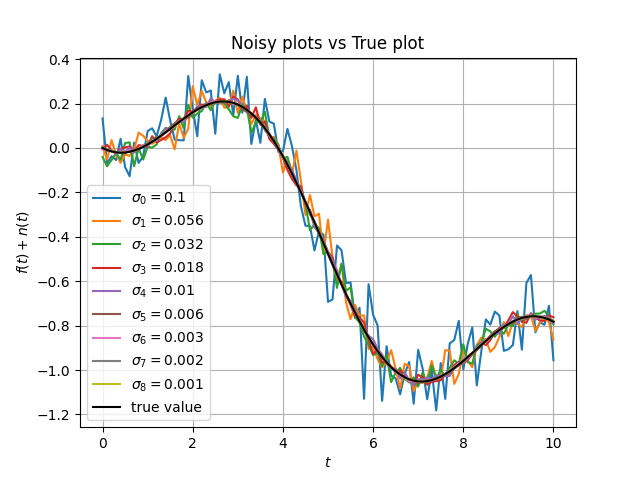
\includegraphics[scale=0.9]{Figure0.png}
                \caption{Noisy Data and True Data (Plot for Q3,Q4)}
                
            \end{figure}
            
            From the above figure it is clear that the noise(deviation from true value) in increasing with increasing standard deviation $\sigma$.\\
            
          \section{Question 5} 
            The graph is plotted using the true data and sampling a few points from the noisy data with fixed standard deviation $\sigma$ = 0.10.
            \begin{figure}[H]
                \centering
                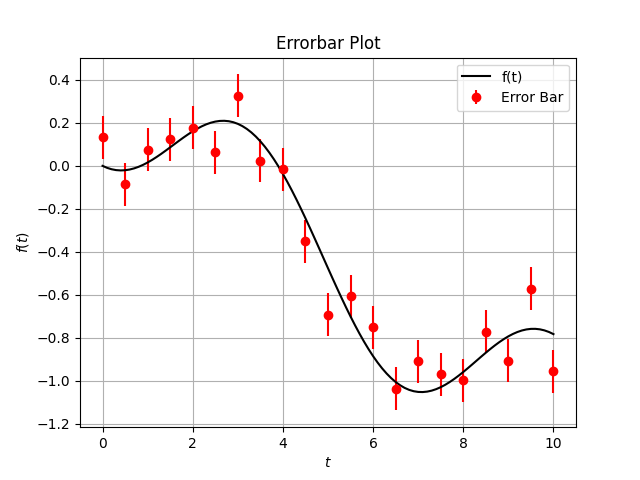
\includegraphics[scale=0.9]{Figure1.png}
                \caption{True Data and sampled Noisy Data (Plot for Q5)}
                
            \end{figure}
            
          \section{Question 6}
            The function {array\_equal}, which returns a boolean value can be used to check for the Equivalence of both the vectors.\\
            Matrix M can be generated by the following:
            \begin{equation}        M = np.c\_[sp.jn( 2, t), t]      \end{equation}   
            The result of follwing will let us know about the equivalence of two vectors:
            \begin{equation} np.array\_equal( g ( t, 1.05, \-0.105) , M.dot(np.array([ 1.05, \-0.105]))) \end{equation}  
            
          \section{Question 8}
            The contour plot of $\epsilon_{ij}$ is plotted in the following Figure 3. There exists \textbf{only one} minima.
            \begin{figure}[H]
                \centering
                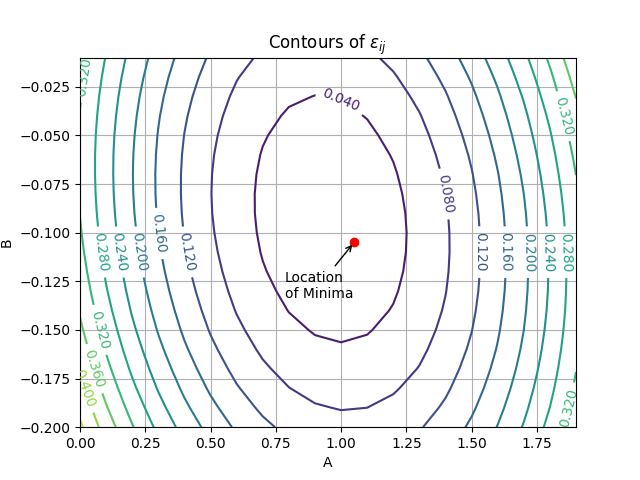
\includegraphics[scale=0.9]{Figure2.png}
                \caption{Contour Plot of the mean squared error versus the parameters A and B(Plot for Q8)}
            \end{figure}            
             
          \section{Question 10}
            The error in the estimate of A and B vs different noise $\sigma$ have been plotted. 
            \begin{figure}[H]
                \centering
                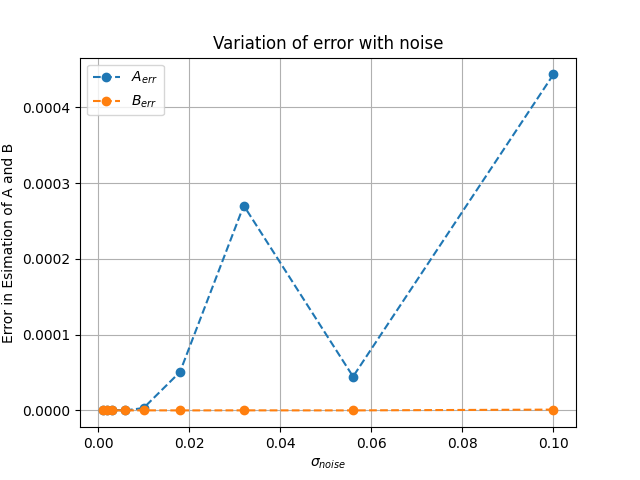
\includegraphics[scale=0.9]{Figure3.png}
                \caption{Error in the estimate of A and B vs different noise $\sigma$(Plot for Q10)}
            \end{figure}            
             The error isn't linear, as it is clear from the graph the increase in error is not uniform with the uniform change with $\sigma$.

          \section{Question 11}
            The error in the estimate of A and B vs different noise $\sigma$ have been plotted using a log-log plot, 
            \begin{figure}[H]
                \centering
                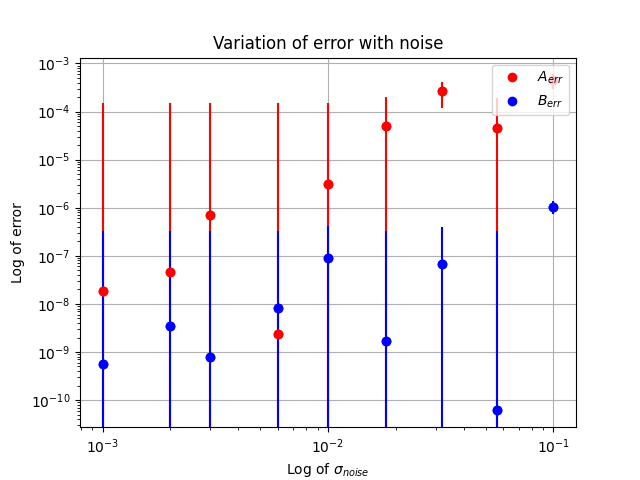
\includegraphics[scale=0.9]{Figure4.png}
                \caption{Log-Log plot of Error in estimate of A and B vs Different noise $\sigma$(Plot for Q10)}
            \end{figure}            
             We can conclude, the error is a better linear fit.
    \section{Conclusion}
        From the above graphs, we can conclude that \textbf{the log of the $\sigma_noise$} is linearly related to \textbf{the log of the error} in the calcuation of the least error fit for a given data.
\end{document}
